\input{"../../../preamble"}

\begin{document}

\title{CSC263-Notes-03-09-2015}

\input{"../csc263-header"}
\rhead{March 9, 2015}

\section*{Lecture 17}

\reversemarginpar
\mpreadings

\noindent 22.2, 22.3 \\

\mpselftest

\noindent 22.3-2

\subsection*{Depth-First Search}

\begin{lstlisting}[mathescape]

DFS(V,E):
	for each v in V:
		colour[v] $\leftarrow$ white
		f[v] $\leftarrow$ d[v] $\leftarrow$ $\infty$
		p[v] $\leftarrow$ NIL
	time $\leftarrow$ 0 # global
	for each v in V:
		if colour[v] = white:
			DFS-Visit(G,v)

DFS-Visit(G=(V,E), u):
	colour[u] $\leftarrow$ gray
	d[u] $\leftarrow$ time $\leftarrow$ time + 1
	for each (u,v) in E:
		if colour[v] == white:
			p[v] $\leftarrow$ u
			DFS-Visit(G,v)
	colour[u] $\leftarrow$ black
	if[u] $\leftarrow$ time $\leftarrow$ time + 1

\end{lstlisting}

\begin{center}
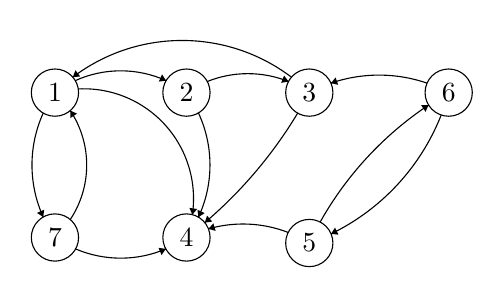
\begin{tikzpicture}[scale=0.1]
\tikzstyle{every node}+=[inner sep=0pt]
\draw [black] (16.6,-14.7) circle (3);
\draw (16.6,-14.7) node {$1$};
\draw [black] (33.3,-14.7) circle (3);
\draw (33.3,-14.7) node {$2$};
\draw [black] (48.9,-14.7) circle (3);
\draw (48.9,-14.7) node {$3$};
\draw [black] (66.6,-14.7) circle (3);
\draw (66.6,-14.7) node {$6$};
\draw [black] (16.6,-33.1) circle (3);
\draw (16.6,-33.1) node {$7$};
\draw [black] (33.3,-33.1) circle (3);
\draw (33.3,-33.1) node {$4$};
\draw [black] (48.9,-33.8) circle (3);
\draw (48.9,-33.8) node {$5$};
\draw [black] (18.867,-12.739) arc (127.1227:52.8773:23.003);
\fill [black] (18.87,-12.74) -- (19.81,-12.65) -- (19.2,-11.86);
\draw [black] (19.179,-13.179) arc (114.38809:65.61191:13.976);
\fill [black] (30.72,-13.18) -- (30.2,-12.39) -- (29.79,-13.3);
\draw [black] (35.941,-13.29) arc (111.88332:68.11668:13.841);
\fill [black] (46.26,-13.29) -- (45.7,-12.53) -- (45.33,-13.46);
\draw [black] (51.646,-13.499) arc (109.03184:70.96816:18.72);
\fill [black] (51.65,-13.5) -- (52.56,-13.71) -- (52.24,-12.77);
\draw [black] (50.278,-31.136) arc (150.66501:123.69235:43.434);
\fill [black] (64.05,-16.28) -- (63.11,-16.3) -- (63.66,-17.14);
\draw [black] (65.65,-17.544) arc (-21.51105:-64.13159:28.31);
\fill [black] (51.66,-32.64) -- (52.6,-32.74) -- (52.17,-31.84);
\draw [black] (47.422,-17.31) arc (-31.03879:-49.54551:56.683);
\fill [black] (35.63,-31.21) -- (36.57,-31.08) -- (35.92,-30.32);
\draw [black] (34.819,-17.282) arc (24.99153:-24.99153:15.666);
\fill [black] (34.82,-30.52) -- (35.61,-30) -- (34.7,-29.58);
\draw [black] (19.557,-14.232) arc (92.83821:-8.38389:13.953);
\fill [black] (34.05,-30.2) -- (34.66,-29.48) -- (33.67,-29.34);
\draw [black] (18.542,-16.978) arc (33.57877:-33.57877:12.516);
\fill [black] (18.54,-16.98) -- (18.57,-17.92) -- (19.4,-17.37);
\draw [black] (15.111,-30.501) arc (-155.56892:-204.43108:15.96);
\fill [black] (15.11,-30.5) -- (15.23,-29.57) -- (14.32,-29.98);
\draw [black] (30.681,-34.552) arc (-66.89225:-113.10775:14.602);
\fill [black] (30.68,-34.55) -- (29.75,-34.41) -- (30.14,-35.33);
\draw [black] (36.088,-32.004) arc (106.04449:68.81703:15.89);
\fill [black] (36.09,-32) -- (37,-32.26) -- (36.72,-31.3);
\end{tikzpicture}
\end{center}

\begin{tabular}{l @{ : } l}
	1 & [2,4,7] \\
	2 & [3.4] \\
	3 & [1,4] \\
	4 & [$\;$] \\
	5 & [4,6] \\
	6 & [3,5] \\
	7 & [1,4]
\end{tabular} \\

\begin{tabular}{c | c | c | c | c }
	v & c & p & d & f \\ \hline
	1 & B &   & 1  & 10 \\
	2 & B & 1 & 2  & 7 \\
	3 & B & 2 & 3  & 6 \\
	4 & B & 3 & 4  & 5 \\
	5 & B &   & 11 & 14 \\
	6 & B & 5 & 12 & 13 \\
	7 & B & 1 & 8  & 9 \\
\end{tabular}

\end{document}
